% No automatic EPS-to-PDF conversion (the figure is a PDF).
\newcommand*{\DoNotLoadEpstopdf}{}
\documentclass[11pt,a4paper]{article}

\usepackage[T1]{fontenc}
\usepackage{lmodern}
\usepackage{microtype}
\usepackage[margin=2.5cm]{geometry}

\newcommand{\PaperTitle}{Edge colorings of plane graphs with facial defect list [1,1,2]}
\newcommand{\PaperAuthor}{Norbert Micheľ}

\usepackage{amsmath}
\usepackage{amssymb}
\usepackage{amsthm}
\usepackage{thmtools}
\usepackage{graphicx}
\usepackage{booktabs}
\usepackage[numbers,sort&compress]{natbib}
\usepackage[hidelinks]{hyperref}
\hypersetup{pdftitle={\PaperTitle}, pdfauthor={\PaperAuthor}}
\usepackage[capitalise,noabbrev]{cleveref}

\declaretheorem[name=Definition,  style=definition, numberwithin=section]{definition}
\declaretheorem[name=Theorem,     style=plain,      sibling=definition]{theorem}
\declaretheorem[name=Lemma,       style=plain,      sibling=definition]{lemma}
\declaretheorem[name=Proposition, style=plain,      sibling=definition]{proposition}
\declaretheorem[name=Corollary,   style=plain,      sibling=definition]{corollary}
\declaretheorem[name=Conjecture,  style=plain,      sibling=definition]{conjecture}
\declaretheorem[name=Remark,      style=remark,     sibling=definition]{remark}

\title{Edge colorings of plane graphs\\ with facial defect list $[1,1,2]$}
\author{\PaperAuthor\\[0.5ex]
  {\normalsize Institute of Computer Science, Faculty of Science}\\
  {\normalsize Pavol Jozef Šafárik University in Košice, Košice, Slovakia}}
\date{Working notes, 13 October 2026}

\begin{document}

\maketitle

\begin{abstract}
Volesková and Fabrici announced that every plane graph has a $[1,2,2]$-edge coloring: three colors, the first without facially adjacent edges, the other two with monochromatic facial paths of at most two edges.
We ask whether a plane graph without a $[1,1,2]$-edge coloring exists.
A computer search finds none among all 77\,274 connected plane graphs with at most eight edges and all 693\,855 3-connected plane graphs with at most 22 edges.
We prove a parity criterion for the third color class, a construction of $[1,1,2]$-edge colorings from two 2-colorings, and the existence for quadrangulations.
With two colors examples exist: we give 3-connected plane graphs without a $[2,2]$-edge coloring and without a $[1,3]$-edge coloring.
The proofs in these notes have not been checked by a second reader.
\end{abstract}

\section{The question}
\label{sec:question}

Let $G$ be a connected plane graph with vertex set $V$, edge set $E$ and face set $F$; loops and multiple edges are allowed.
A \emph{corner} of $G$ is a pair of consecutive edges of the boundary walk of a face $f$, taken with the vertex $v$ between them; it is a corner of $v$ and of $f$.
Two distinct edges are \emph{facially adjacent} if they form a corner.
A \emph{facial trail} is a sequence of pairwise distinct edges that are consecutive on the boundary walk of a face.
A facial trail with $k$ edges is a \emph{facial path} if the $k+1$ vertices it passes are pairwise distinct.

\begin{definition}[Defect list]
\label{def:defect}
Let $d_1,\dots,d_k$ be positive integers.
A coloring of $E$ with the colors $1,\dots,k$ is a \emph{$[d_1,\dots,d_k]$-edge coloring} if, for every color $i$, no facial trail with $d_i+1$ edges has all its edges of color $i$.
A coloring of $V$ with the colors $1,\dots,k$ is a \emph{$[d_1,\dots,d_k]$-vertex coloring} if, for every color $i$, no $d_i+1$ pairwise distinct vertices that are consecutive on a boundary walk have all color $i$.
\end{definition}

A color with $d_i=1$ has no two facially adjacent edges.
The abstract of Volesková~\cite{Voleskova2026FacialDefect} bounds monochromatic paths, so for $d_i\ge 2$ it forbids only facial paths; we call this the \emph{path reading} and \cref{def:defect} the \emph{trail reading}.
The two readings differ on faces of length three and on boundary walks that repeat a vertex.
Every coloring that is valid in the trail reading is valid in the path reading.
We therefore state existence in the trail reading and non-existence in the path reading whenever we can.

The following is known.
Every plane graph has a $[1,1,1,1]$-edge coloring, by the Four Color Theorem~\cite{AppelHaken1976}, and a wheel has no $[1,1,1]$-edge coloring~\cite[p.~631]{Czap2019FacialRST}.
Every plane graph has a $[1,2,2]$-edge coloring~\cite{Voleskova2026FacialDefect}; the abstract gives no proof.
Every plane graph has a $[2,2,2]$-vertex coloring~\cite[Theorem~3]{Jendrol2026ThreeColoring}, with the proof corrected in~\cite{Jendrol2026Corrigendum}, and no $4$-chromatic plane graph has a $[1,1,1]$-vertex coloring.
The list between the theorem and the counterexample is $[1,1,2]$.

\medskip
\noindent\textbf{Question.} Is there a plane graph without a $[1,1,2]$-edge coloring?
\medskip

A positive answer would show that the list $[1,2,2]$ is best possible.
\Cref{sec:search} reports that no small graph answers the question.
\Cref{sec:criterion} characterizes the sets of edges that can form the third color class, and \cref{sec:two-colors} gives the examples for two colors.

The abstract~\cite{Voleskova2026FacialDefect} also announces a $[1,1,1,2,2]$-total coloring of every plane graph and does not define the defect of a total coloring.
We test only colorings of $V\cup E$ in which the vertices and the edges separately satisfy \cref{def:defect} and every vertex differs from its incident edges.
For the list $[1,1,1,1,1]$ this is the facial total-coloring with five colors, which is conjectured to exist for every plane graph~\cite[Conjecture~15]{Czap2019FacialRST}; six colors suffice~\cite[Theorem~14]{Czap2019FacialRST}.

\section{Computer search}
\label{sec:search}

We examined three sets of graphs.
\begin{itemize}
  \item[(M)] All connected plane graphs with at most eight edges, loops and multiple edges allowed, up to homeomorphisms of the sphere: 77\,274 graphs.
        They arise from one edge by adding pendant edges and chords of faces; a canonical code of the rotation system removes isomorphic copies.
  \item[(P)] All 3-connected plane graphs with at most 22 edges: 693\,855 graphs.
        They arise from the wheels by adding edges and splitting vertices, which gives every 3-connected graph by Tutte's wheel theorem~\cite[Notes of Chapter~3]{Diestel2025}.
  \item[(R)] 2\,800\,000 random plane graphs with 10 to 45 edges, grown by random pendant edges and chords.
\end{itemize}
The numbers of graphs with each number of edges in (M) and (P) agree with the sequences A006385 and A002840 of~\cite{OEIS}.
A backtracking search with unit propagation decides each coloring.
A second program, written separately, repeated the counts of \cref{tab:smallest} on the graphs of (M) and on the examples of \cref{sec:two-colors}.
The run over the 4\,820\,218 plane graphs with nine and ten edges was not finished when these notes were written.

\begin{proposition}[Computer search]
\label{prop:search}
In the trail reading, every graph in the sets (M), (P) and (R) has a $[1,1,2]$-edge coloring and a $[1,1,2]$-vertex coloring.
Every graph in (M) and (P) has a facial total-coloring with five colors.
\end{proposition}

A plane graph without a $[1,1,2]$-edge coloring, if one exists, therefore has at least nine edges, and at least 23 edges if it is 3-connected.
The same bounds hold for the vertex version, where the list $[1,1,2]$ would strengthen the theorem of Jendroľ~\cite{Jendrol2026ThreeColoring}.

\begin{table}[ht]
\centering
\caption{The smallest number of edges of a graph without the coloring; a dash means that every graph of the set has one.}
\label{tab:smallest}
\begin{tabular}{@{}llcc@{}}
\toprule
Coloring & Reading & In (M) & In (P) \\
\midrule
$[1,1,1]$-edge   & both  & 4  & 8  \\
$[1,1,2]$-edge   & trail & -- & -- \\
$[1,2]$-edge     & trail & 5  & 8  \\
$[1,2]$-edge     & path  & 6  & 11 \\
$[2,2]$-edge     & trail & -- & 15 \\
$[2,2]$-edge     & path  & -- & 21 \\
$[1,3]$-edge     & trail & 8  & 15 \\
$[1,3]$-edge     & path  & -- & 18 \\
$[2,3]$-, $[3,3]$-, $[1,4]$-edge & trail & -- & -- \\
\midrule
$[1,1,1]$-vertex &       & 6  & 6  \\
$[1,1,2]$-vertex &       & -- & -- \\
$[2,2]$-vertex   &       & -- & 15 \\
$[1,3]$-vertex   &       & -- & 17 \\
$[2,3]$-, $[3,3]$-, $[1,4]$-vertex & & -- & -- \\
\bottomrule
\end{tabular}
\end{table}

\section{A criterion for the third color class}
\label{sec:criterion}

A set $S\subseteq E$ is \emph{admissible} if the edges of $E\setminus S$ can be colored with two colors so that facially adjacent edges get different colors.
It is \emph{trail-free} if it contains no facial trail with three edges.
The third color class of a $[1,1,2]$-edge coloring is an admissible trail-free set, and every admissible trail-free set is such a class.
A superset of an admissible set is admissible.

The elements of $X=V\cup F$ are the \emph{nodes} of $G$.
The \emph{weight} $w(x)$ of a node $x$ is the number of corners of $x$ that are formed by two distinct edges.
It equals the degree of a vertex and the length of a face, unless the vertex has degree one or the face has length one.
For $S\subseteq E$ let $H_S$ be the graph on $X$ in which the two ends and the two sides of every edge of $S$ are pairwise adjacent.

\begin{theorem}[Parity criterion]
\label{thm:parity}
Let $G$ be a connected plane graph and let $S\subseteq E$.
The set $S$ is admissible if and only if, in every component of $H_S$, the sum of the weights of the nodes is even.
\end{theorem}

\begin{proof}
Let $M$ be the plane graph with vertex set $E$ that has one edge for every corner of $G$, joining the two edges of the corner and drawn inside the corner.
Every face of $M$ contains exactly one node of $G$, and the edge of $M$ in a corner of a vertex $v$ and a face $f$ separates the face of $v$ from the face of $f$.
Let $B$ be the graph obtained from $M$ by deleting the vertices in $S$ and the loops.
Two edges of $E\setminus S$ are facially adjacent if and only if they are adjacent in $B$, so $S$ is admissible if and only if $B$ is bipartite.

A plane graph is bipartite if and only if every face has an even number of incidences with edges, an edge with the same face on both sides counted twice.
Indeed, in a bipartite graph every boundary walk is even.
Conversely, the components of the graph and its faces form a tree in which a component and a face are adjacent if a boundary walk of the face lies in the component.
The lengths of the boundary walks around one face have an even sum by assumption, and those around one component sum to twice its number of edges.
Removing leaves of the tree one by one shows that every boundary walk is even, and a connected plane graph with even boundary walks is bipartite.

The faces of $B$ are unions of faces of $M$.
Deleting a vertex $e\in S$ removes the corners at the two ends of $e$ on its two sides and thus unites the faces of the two ends and of the two sides of $e$.
Deleting a loop of $M$ unites the face of a node of weight zero with one other face.
Hence the nodes in a face $\Phi$ of $B$ form a component $K$ of $H_S$ together with nodes of weight zero.
Let $b(x)$ be the number of corners of a node $x$ that are edges of $B$.
The number of incidences of $\Phi$ with edges is $\sum_{x\in K} b(x)$.
A corner counted in $w(x)-b(x)$ is formed by two distinct edges, one of them in $S$; its vertex and its face are adjacent in $H_S$, so the corner is counted for two nodes of $K$.
Therefore $\sum_{x\in K} b(x)$ and $\sum_{x\in K} w(x)$ have the same parity.
\end{proof}

A node of odd weight thus needs an edge of $S$ at it, and the edges of $S$ have to join the odd nodes in groups of even size.
In the theta graph with three paths of three edges, the two vertices of degree three are the only odd nodes.
One edge at each of them, on a common face and not on a common path, form an admissible trail-free set.

\begin{proposition}[Product construction]
\label{prop:product}
Let $\sigma\colon V\to\{0,1\}$ and $\tau\colon F\to\{0,1\}$, and let $N$ be the set of edges whose ends differ in $\sigma$ and whose sides differ in $\tau$.
Then $E\setminus N$ is admissible.
\end{proposition}

\begin{proof}
For an edge of $N$ directed from $x$ to $y$ with the face $f$ on its left, the value $\sigma(x)+\tau(f)$ modulo two does not depend on the direction, because the other direction changes both summands.
Color the edge by this value.
Let two edges of $N$ form a corner of a vertex $v$ and a face $f$, and direct both away from $v$.
The face $f$ lies on the left of one of them and on the right of the other, whose left side has the other value of $\tau$.
The two edges get different colors.
\end{proof}

The set $N$ of \cref{prop:product} is the intersection of an edge cut with the boundary of a set of faces.
Every 3-connected plane graph with at most 22 edges has functions $\sigma$ and $\tau$ for which $E\setminus N$ is trail-free.
The theta graph above has none: two of its three faces get the same value of $\tau$, and the three edges of their common path lie in $E\setminus N$.

\begin{corollary}
\label{cor:quadrangulation}
Every 2-edge-connected plane graph in which every face has length four has a $[1,1,2]$-edge coloring in the trail reading.
\end{corollary}

\begin{proof}
All faces are even, so the graph is bipartite; let $\sigma$ be a proper 2-coloring of the vertices.
Choose $\tau$ with the largest number of edges whose sides differ in $\tau$.
No edge has the same face on both sides, so changing $\tau$ on one face $f$ exchanges the edges of $f$ whose sides differ with those whose sides agree.
By the choice of $\tau$, at least two of the four edges of $f$ have sides that differ.
A facial trail with three edges of $f$ misses one edge of $f$ and thus contains an edge of $N$.
By \cref{prop:product}, the set $E\setminus N$ is admissible and trail-free.
\end{proof}

Plane triangulations and bridgeless cubic plane graphs have $[1,1,1]$-edge colorings, which is Tait's form of the Four Color Theorem~\cite[p.~631]{Czap2019FacialRST}.

\begin{proposition}[Reduction]
\label{prop:reduction}
Let $e$ be an edge of $G$, and let $G'$ be $G-e$ if $e$ is not a bridge or $G/e$ if $e$ is not a loop.
If $S'$ is an admissible trail-free set of $G'$ and no facial trail of $G$ with three edges lies in $S'\cup\{e\}$ and contains $e$, then $S'\cup\{e\}$ is an admissible trail-free set of $G$.
A graph without a $[1,1,2]$-edge coloring that has the fewest edges has no vertex of degree one and no face of length one.
\end{proposition}

\begin{proof}
Two edges other than $e$ that form a corner of $G$ form a corner of $G'$, and a facial trail of $G$ that avoids $e$ is a facial trail of $G'$.
This proves the first statement.

Let $u$ be a vertex of degree one with the edge $e=uv$, let $G'=G/e$ and let $S'$ be an admissible trail-free set of $G'$.
The boundary walk through $e$ reads $\dots,q',q,e,e,p,p',\dots$, and the facial trails with three edges through $e$ are $(q',q,e)$ and $(e,p,p')$.
If one of them lies in $S'\cup\{e\}$, then $q\in S'$ or $p\in S'$.
The edge $e$ is facially adjacent only to $q$ and $p$, so at most one edge of $E\setminus S'$ is facially adjacent to $e$, and $S'$ is an admissible trail-free set of $G$.

Let $e$ be a loop that bounds a face of length one and let $G'=G-e$.
The boundary walk of the other face at $e$ reads $\dots,q',q,e,p,p',\dots$; each of the three facial trails with three edges through $e$ contains $q$ or $p$, and $e$ is facially adjacent only to $q$ and $p$.
The argument of the previous case applies.
\end{proof}

\section{Two colors}
\label{sec:two-colors}

For vertices, two colors with the list $[4,4]$ always suffice, the list $[3,3]$ is conjectured to suffice and the list $[2,2]$ fails~\cite[Theorems~1 and~4, Conjecture~3]{Czap2021FacialPaths}.
We found no published statement for edges.
\Cref{tab:smallest} shows that the lists $[2,2]$ and $[1,3]$ fail for edges in both readings.

\begin{proposition}[Computer search]
\label{prop:two-colors}
The graph of \cref{fig:two-color-examples}(a) has no $[2,2]$-edge coloring and the graph of \cref{fig:two-color-examples}(b) has no $[1,3]$-edge coloring, in either reading.
Both have $[1,1,2]$-edge colorings, the first has a $[2,3]$-edge coloring and the second a $[1,4]$-edge coloring.
\end{proposition}

\begin{figure}[ht]
\centering
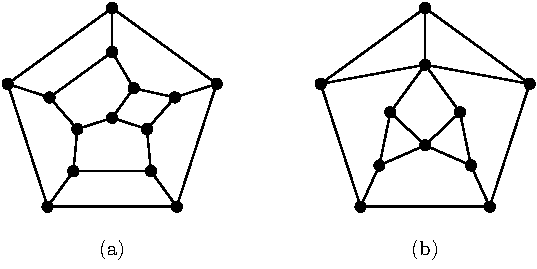
\includegraphics{two-color-examples}
\caption{Plane graphs with no $[2,2]$-edge coloring (a) and no $[1,3]$-edge coloring (b).}
\label{fig:two-color-examples}
\end{figure}

The graph (a) is cubic with 14 vertices, and the graph (b) has 11 vertices and 18 edges.
Among 3-connected plane graphs, (a) is the only one with at most 21 edges without a $[2,2]$-edge coloring in the path reading, and no graph with fewer than 18 edges lacks a $[1,3]$-edge coloring in the path reading.

\section{Open questions}
\label{sec:open}

\begin{conjecture}
\label{thm:conjecture-edge}
Every plane graph has a $[1,1,2]$-edge coloring.
\end{conjecture}

The conjecture rests on \cref{prop:search}, and by \cref{thm:parity} it asks for a trail-free set of edges that joins the nodes of odd weight in groups of even size.

\begin{conjecture}
\label{thm:conjecture-vertex}
Every plane graph has a $[1,1,2]$-vertex coloring.
\end{conjecture}

For plane triangulations \cref{thm:conjecture-vertex} follows from the Four Color Theorem: two of the four color classes are merged, and no face is monochromatic.
We do not know whether two colors with the list $[2,3]$ suffice for edges, or whether every 3-connected plane graph has functions $\sigma$ and $\tau$ as in \cref{prop:product} with $E\setminus N$ trail-free.

\bibliographystyle{plainnat}
\bibliography{references}

\end{document}
